\chapter{Development Process}
\label{ch:development_process}

This chapter details the process of translating stakeholder needs into a functioning dashboard application. It covers prioritization of requirements, technology selection, planning, iterative development, and testing activities. It also reflects on practical choices made throughout development, supported by figures.

%Her var alt av requirements, det er nå flyttet til resultat. Kopi i x4 som vi kan brukes videre til 'discussion'.


\section{Application Status: End of Development Process}
\label{sec:status_at_completion}
tekst om hele prosessen som kommer under

\subsection{System Design}
\label{subsec:system_design}
The figure below shows all the different pages and options the user has, to give an overview of the application before discussing logic and moving on to component specifics and design choices.

%figur av hele siden oppsumert
\begin{figure}[htbp]
        \centering
        \includegraphics[width=\textwidth]{figures/Sitemap.png}
        \caption{Sitemap}
        \label{fig:sitemap}
\end{figure} 

\subsubsection{Monitoring Logic}
\label{subsubsec:monitoring_logic}
The monitoring system was implemented using \gls{axios} and \gls{cron}. Each monitored website was checked at a user-defined interval, with scheduled jobs executing \acrshort{http} requests to collect two key metrics: the \acrshort{http} status code and the response time to the first byte. These values were stored in the database for further processing.

Collected data was used to generate uptime statistics and response time charts within the user interface. The monitoring logic relied exclusively on the \acrshort{http} status code and timing information provided by \gls{axios} to determine whether a website was considered up or down.

If a timeout occurred during a check, the result was marked as failed (red) in the system. A follow-up check was automatically scheduled 60 seconds later to verify whether the issue persisted. If the second check also failed, an incident is created, and an alert with subsequent email notification was sent if the user had alerts enabled for that website.

In addition to downtime alerts, users could define custom thresholds for acceptable response times. If a site exceeded this threshold, a "slow" alert was created. These thresholds were configurable per website, allowing users to adjust expectations for sites that consistently load more slowly.

\subsubsection{Alert System}

The alert system was integrated into the scheduled monitoring jobs. When regular monitoring check for any given website failed, the backend evaluated whether the failure met the criteria for triggering an alert. These criteria included threshold conditions defined by the user, such as consecutive failures or prolonged downtime.

Once the conditions were met, an alert record was created in the database. 
The backend server the  sends an email to a user specified email-address for that website, if the user has alerts configured. To prevent sending unnecessary alerts, the system only allowed for one active alert per website for each user. The user had to manually delete an alert to receive a new one.

% stemmer for å fjerne dette nå, flyttet incident teori ned til dashboard

The alert system is designed in a way not to only notify users of issues, but also to do so in a manner that supports usability, clarity, and minimizes cognitive load. Achieving this is done by designing the system in line with Stephen Few's principles of simplicity and critical value exceptions ( see \autoref{subsubsec:principle_simplicity}. Rather than overwhelming the user with every failure, the system uses threshold conditions, both user-defined and system standard. This approach ensures that only meaningful anomalies surface, aligning with Few's suggestions that dashboards should highlight actionable information without excessive clutter. The alert logic reinforces Don Norman's principle of constraints by preventing redundant alerts, guiding user attention, and reducing unnecessary interruptions (see \autoref{par:constraints}. 

\subsubsection{Incidents System}
After \hyperref[subsec:user_testing]{user test 2}, which focused on application flow, the team received feedback explaining that test subjects wanted a better way to identify why a red/orange status indicator was displayed. This led to a new functional requirement F.11 being written, to develop an incident system.

The incident system works by adding an incident to the database if a monitored website has been down or slow for two consecutive checks. This moves the dashboard card  for that website to the top of the Dashboard, as well as displaying a yellow/red status indicator depending on the severity of the incident (down/slow). Past and present incidents can be displayed in a list on a separate page, or for a specific website by clicking on corresponding card on the dashboard.

\subsubsection{User Authentication}
As described in \autoref{sec:def_req}, user authentication was not originally a requirement for the application. However, after feedback gathered during the requirement elicitation process, it was deemed beneficial that users could have their own dashboard with custom websites, instead of one central dashboard that everyone had access to. Based on this, a robust authentication system using \textbf{\gls{jsonwebtoken}} was implemented. This enabled user registration and login/logout functionality, as well as each user only having access to their own personal dashboard.




\subsection{Implementation}
This section outlines the core React components used in the frontend, focusing on their responsibilities, interactions, and design rationale.

The implementation draws directly on the design theories discussed in Chapter~\ref{ch:theory}. Layout and data prioritization were guided by Few’s dashboard principles (\autoref{subsec:principles_of_dashboard_design}), emphasizing clarity, simplicity, and the visibility of critical information. Interaction patterns follow Norman’s principles of affordance, feedback, and visibility (\autoref{subsubsec:don_norman_design_principles}), shaping how users engage with the system. Nielsen’s heuristics (\autoref{subsubsec:connecting_visual_and_interaction_design}) informed the use of consistency, status indicators, and error handling.

Together, these frameworks supported the development of a frontend that is both functional and user-friendly, grounded in established design theory.



\subsubsection{Dashboard Page}
The dashboard page serves as the main interface of the application. It displays near real-time data on website availability and uptime statistics, acting as the central point of user interaction (see \ref{sec:website_monitoring}). In line with Stephen Few's definition, the dashboard is designed to present the most important information in a clear and concise way on a single screen, so the user can monitor important information at a glance, as stated in \ref{subsec:what_is_dashboard}. 

\paragraph{Dashboard Behavior}

The dashboard is the first screen users see after logging in and is where they are expected to spend most of their time. It supports operational monitoring by immediately highlighting when something requires attention. This aligns with Few's concept of critical value exceptions (see \ref{subsubsec:principle_simplicity}), clearly showcasing when user action is needed, and is supported by Nielsen's principle of visibility of system status, which says the system should always keep users informed about what's going on (see \ref{par:visibility_system_status}). 

\paragraph{Dashboard Layout and Design}
The layout applies several of the Gestalt principles, which Few integrates in his theory of dashboard design, as outlined in Section \ref{subsubsec:gestalt_principles}, to organize and simplify the presentation of information. The principle of proximity is used for related data, like uptime and number of incidents, being placed close together to show they belong together. The principle of enclosure, where bordered and shaded sections are used to group data, making the page easier to scan. Using the principle of similarity, with consistent use of fonts, icons, and spacing to reinforce visual coherence. This also supports Norman's principle of consistency by helping users form a predictable mental model of the interface (see \ref{subsubsec:don_norman_design_principles}).

The principle of simplicity is a key focus throughout (see \ref{subsubsec:principle_simplicity}) development. We aim to minimize clutter, using summaries and graphs instead of full data tables and only highlighting detailed data when necessary. This helps to reduce cognitive load and allows users to understand the most critical information quickly

Colour theory is applied deliberately throughout the application (see \ref{subsec:colour_theory}). Warm colours like red and orange are used to indicate warnings or issues that need attention, while cool colours like green and blue indicate stability or success. Complementary colour pairs, such as red and green, are used to create strong visual contrast between positive and negative states. This not only enhances visibility but draws the users attention where it's needed the most. These choices follow traditional colour psychology and support Nielsen's visibility of system status heuristic, helping users immediately understand what is functioning correctly and what requires action (see \ref{par:visibility}).

Instead of treating all monitored websites equally on the dashboard, the system elevates cards representing websites with active incidents. Giving these anomalies visual priority, both through repositioning and color indicators, supports Few's critical value exception (see \ref{subsubsec:principle_simplicity}.

From a visual design perspective, the relocation of the Website Card component reinforces the Gestalt principle of proximity by grouping the most critical elements at the top of the interface. This dynamic update of the interface is supported by Nielsen's heuristic of system status visibility. By clearly informing the user that the system has detected an issue and communicating this change in real time, the dashboard improves both usability and situational awareness, allowing users to focus attention where it is most needed (see \ref{par:visibility_system_status}.

In terms of interaction, several of Norman's principles (\ref{subsubsec:don_norman_design_principles}) are actively applied:

\begin{itemize}
    \item \textbf{Feedback:} The interface gives immediate visual responses to user actions, such as highlighting or updating components in real-time. For example, hovering over the graph for response times reveals tooltips with detailed values.
    \item \textbf{Affordance:} Interactive elements, like the filter field, sort menu, and new website card, use visual cues (icons, shadows, hover effects) to indicate their functionality. This makes their purpose intuitive even without explicit instructions.
    \item \textbf{Visibility:} Core system actions and status indicators are placed front and center, such as overall website status, uptime, incident, or change in website status, ensuring that users can immediately interpret the monitoring state without effort.
    \item \textbf{Consistency:} The cards for each website are identically structured, and repeated UI components behave the same across the dashboard. This reduces the learning curve and improves usability.
\end{itemize}

Together, these design and interaction principles ensure that the dashboard is not only visually clean but also intuitive and easy to use.
    

\subsubsection{Website Card Component}
\label{subsubsec:website_card}

\paragraph{Website Card Behavior}

The website card is a core UI component responsible for displaying the real-time status of a single monitored website. It receives props, such as URL, \acrshort{http} status, last response time, and a list of recent checks, all passed from the backend via API calls.

The component conditionally renders its UI based on the received data.
If the \acrshort{http} status indicates downtime, the card communicates this with a red "Offline" label and a critical warning message. If the site is online, the card displays key metrics such as response time and uptime percentage for the last 24 hours. The visual state of the card updates automatically when new monitoring data arrives from the backend server.



\paragraph{Website Card: Layout and Design}
\label{par:website_card_design}

The website card is designed to communicate status clearly and efficiently. Following Stephen Few's dashboard design principles the component presents a compact, information-rich summary of a website's operational state. By avoiding information overload and using visual prioritization, the component allows users to quickly interpret a site's status at a glance, which is essential for an operational dashboard (see, \ref{subsubsec:different_types_dashboards}). 

Related metrics such as response time, uptime percentage, and current status are close together within the card. This supports the Gestalt principle of proximity, helping users visually connect related data points without cognitive effort. 

The visual design of the website card also benefits from consistent styling across all cards. Typography, iconography, and layout are kept uniform, which reinforces predictability and aligns with Nielsen's heuristic of consistency of standards (see \ref{par:consistency_and_standards}). This helps users build a mental model that applies across cards, regardless of which website is being monitored. 

Colour, together with relevant data or icons, is an essential part of how the website card communicates website status. A green badge signal that a website is operational, orange highlights slower response time, and red indicates downtime or failure. These colours are chosen for their intuitive emotional associations and strong contrast, supporting rapid interpretation. 

Together, these visual and behavioral design choices ensure that each website card contributes meaningfully to the overall usability of the dashboard. Supporting quick decision making and continuous system awareness.


\begin{figure}[H]
    \centering
    \includegraphics[width=1\linewidth]{figures//MVP-dashboard/MVP-cards.png}
    \caption{Visual comparison of the Website Card component in online and offline states}
    \label{fig:websitecard-comparison}
\end{figure}



\subsubsection{Website Details Page}
The Website Details page is one of the main views of the application. It provides more detailed information for a specific website than what is shown on the main dashboard.

\paragraph{Page Behavior}
Users access this page by clicking on a Website Card component. Once navigated, the page dynamically renders several charts and UI elements to present detailed monitoring data fetched from the database. This interaction is outlined in the sequence diagram below (see \autoref{fig:sequence_diagram}).

\begin{figure}[htbp]
        \centering
        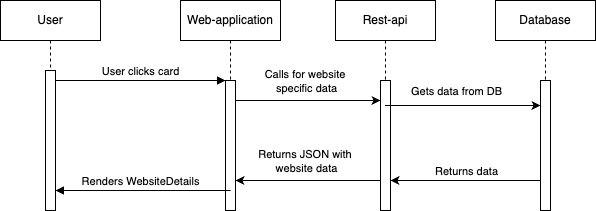
\includegraphics[width=\textwidth]{figures/Sequence_diagram.jpg}
        \caption{Website Details Sequence Diagram}
        \label{fig:sequence_diagram}
\end{figure}

\paragraph{Website Details: Layout and Design}

According to Stephen Few, a dashboard should make it as easy and seamless as possible to find the information needed to take action (see \ref{subsec:what_is_dashboard}). This idea guided the development of the Website Details page. While the dashboard itself is designed to notify users that action is required, the Website Details page is intended to help users understand what action to take.

To support this, the page displays detailed information about recent incidents, as well as historical data on uptime and response time. These are presented through clear and compact visualizations that makes it easy to interpret patterns and spot anomalies. This follows Few's principles to minimizing cognitive load and making critical information visually accessible at a glance (see \ref{subsubsec:principle_simplicity}.

When an incident is active, a large banner appears at the top of the page, pushing other components down. This draws immediate attention using a combination of icons, descriptive text, and strong color contrasts. 

Interactive elements such as buttons and dropdown filters are designed with Don Norman's principle of affordance in mind (see \ref{par:affordance} Their shape, labeling and visual style suggest their function clearly, helping users understand how to interact with the interface. The layout also reflects Jakob Nielsen's usability heuristics (see \ref{subsubsec:connecting_visual_and_interaction_design}. The system's status is always visible through updated status indicators and live chats, ensuring that users are kept informed. The use of consistent styles, icons, and layout patterns across the application reduces confusion and supports a more user-friendly experience. 


\begin{figure}[H]
    \centering
    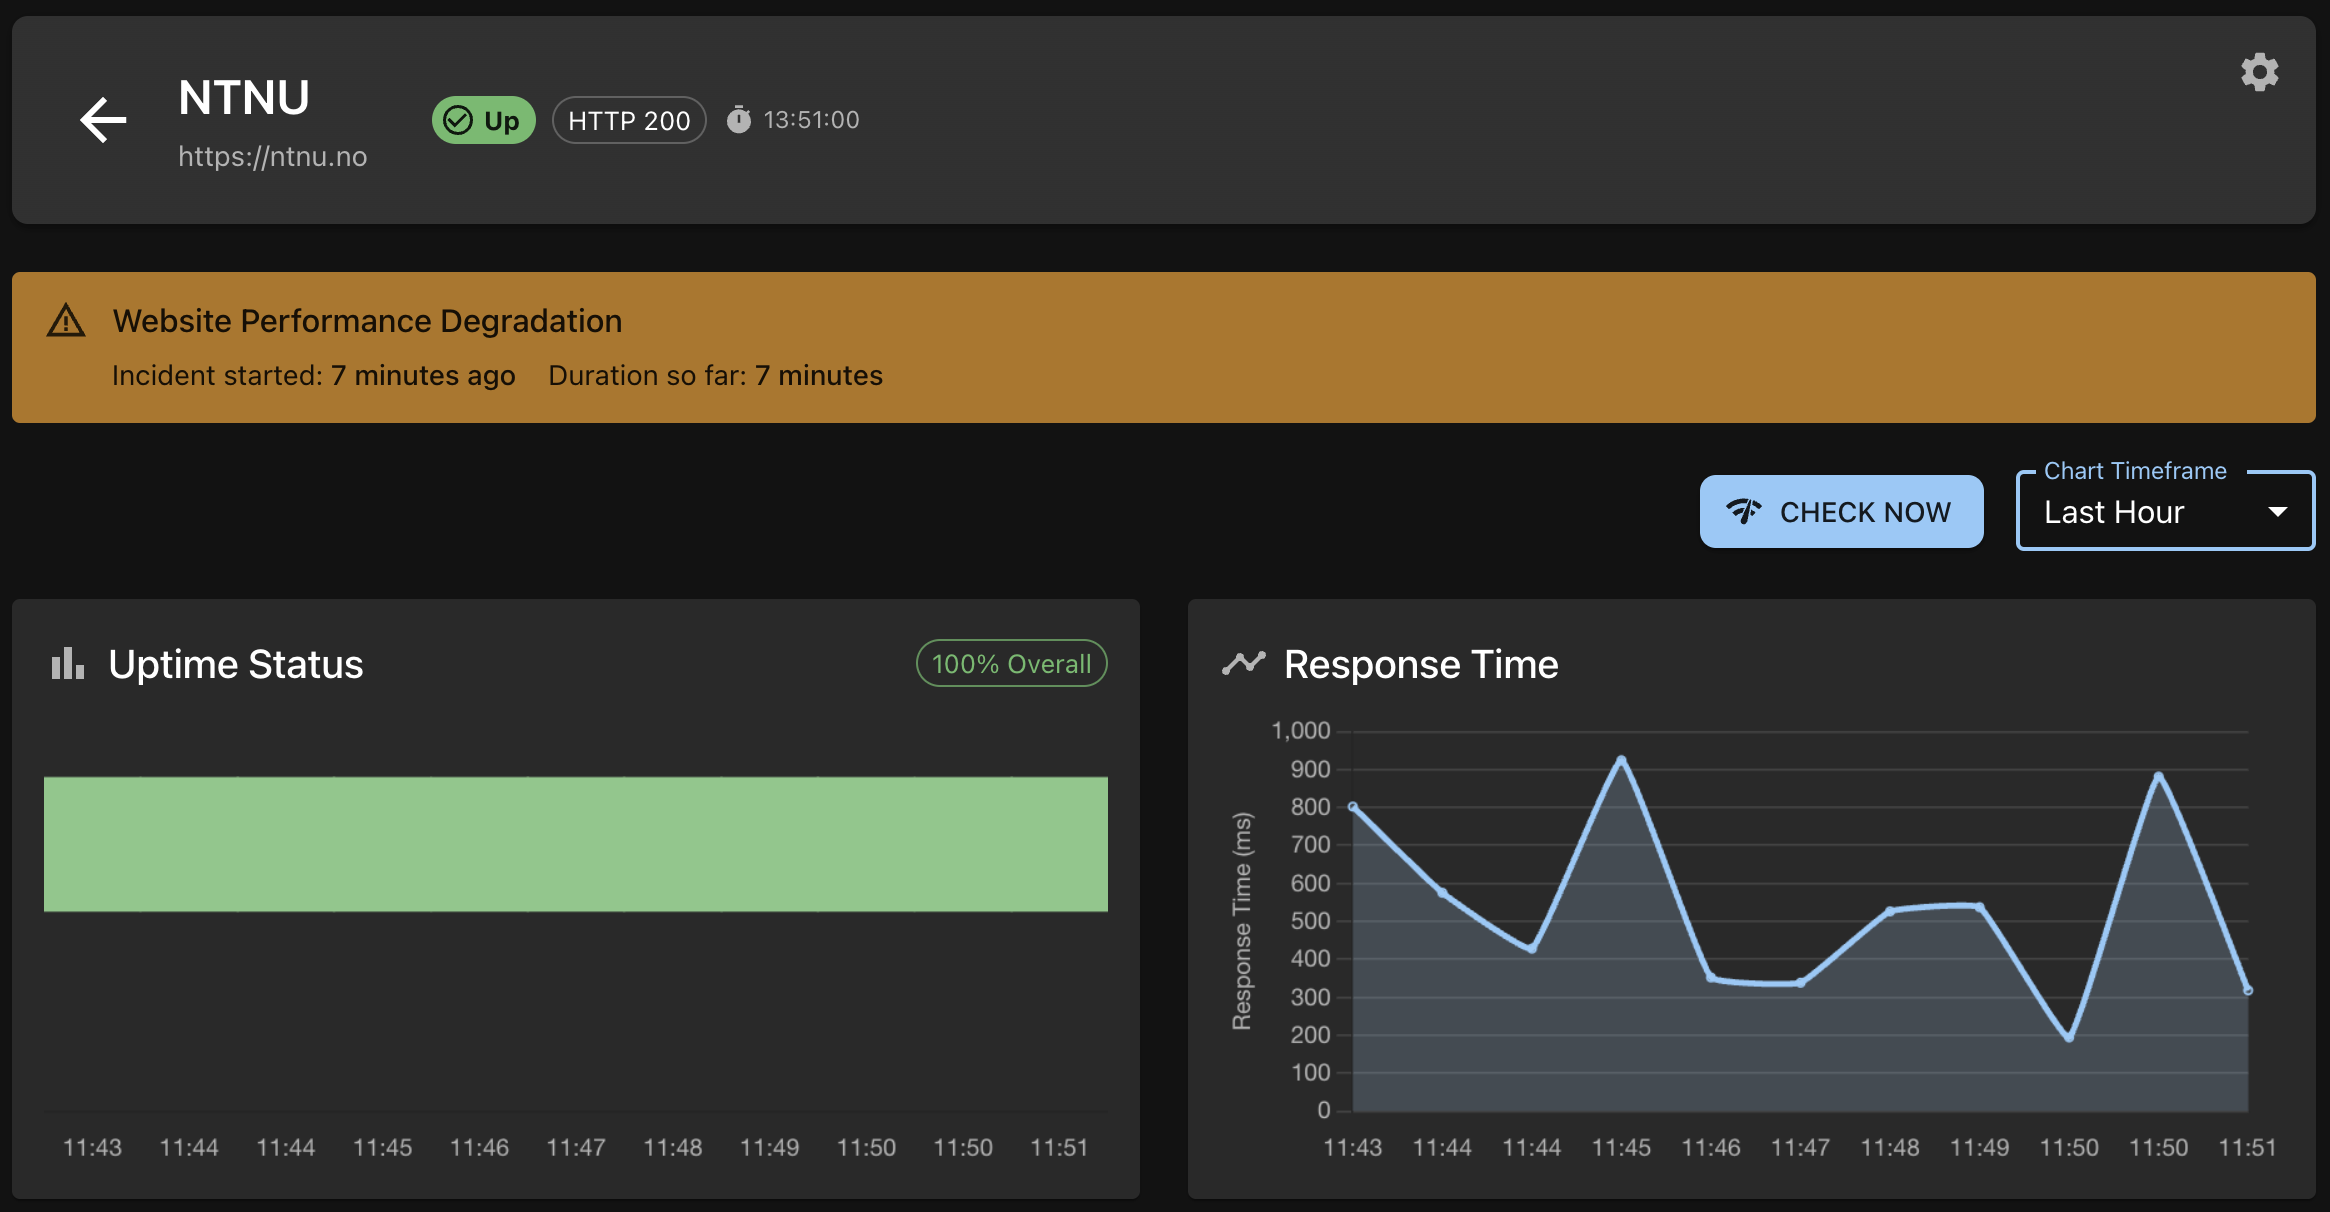
\includegraphics[width=1\linewidth]{figures/websiteDetails.png}
    \caption{Enter Caption}
    \label{fig:enter-label}
\end{figure}


\begin{figure}[H]
    \centering
    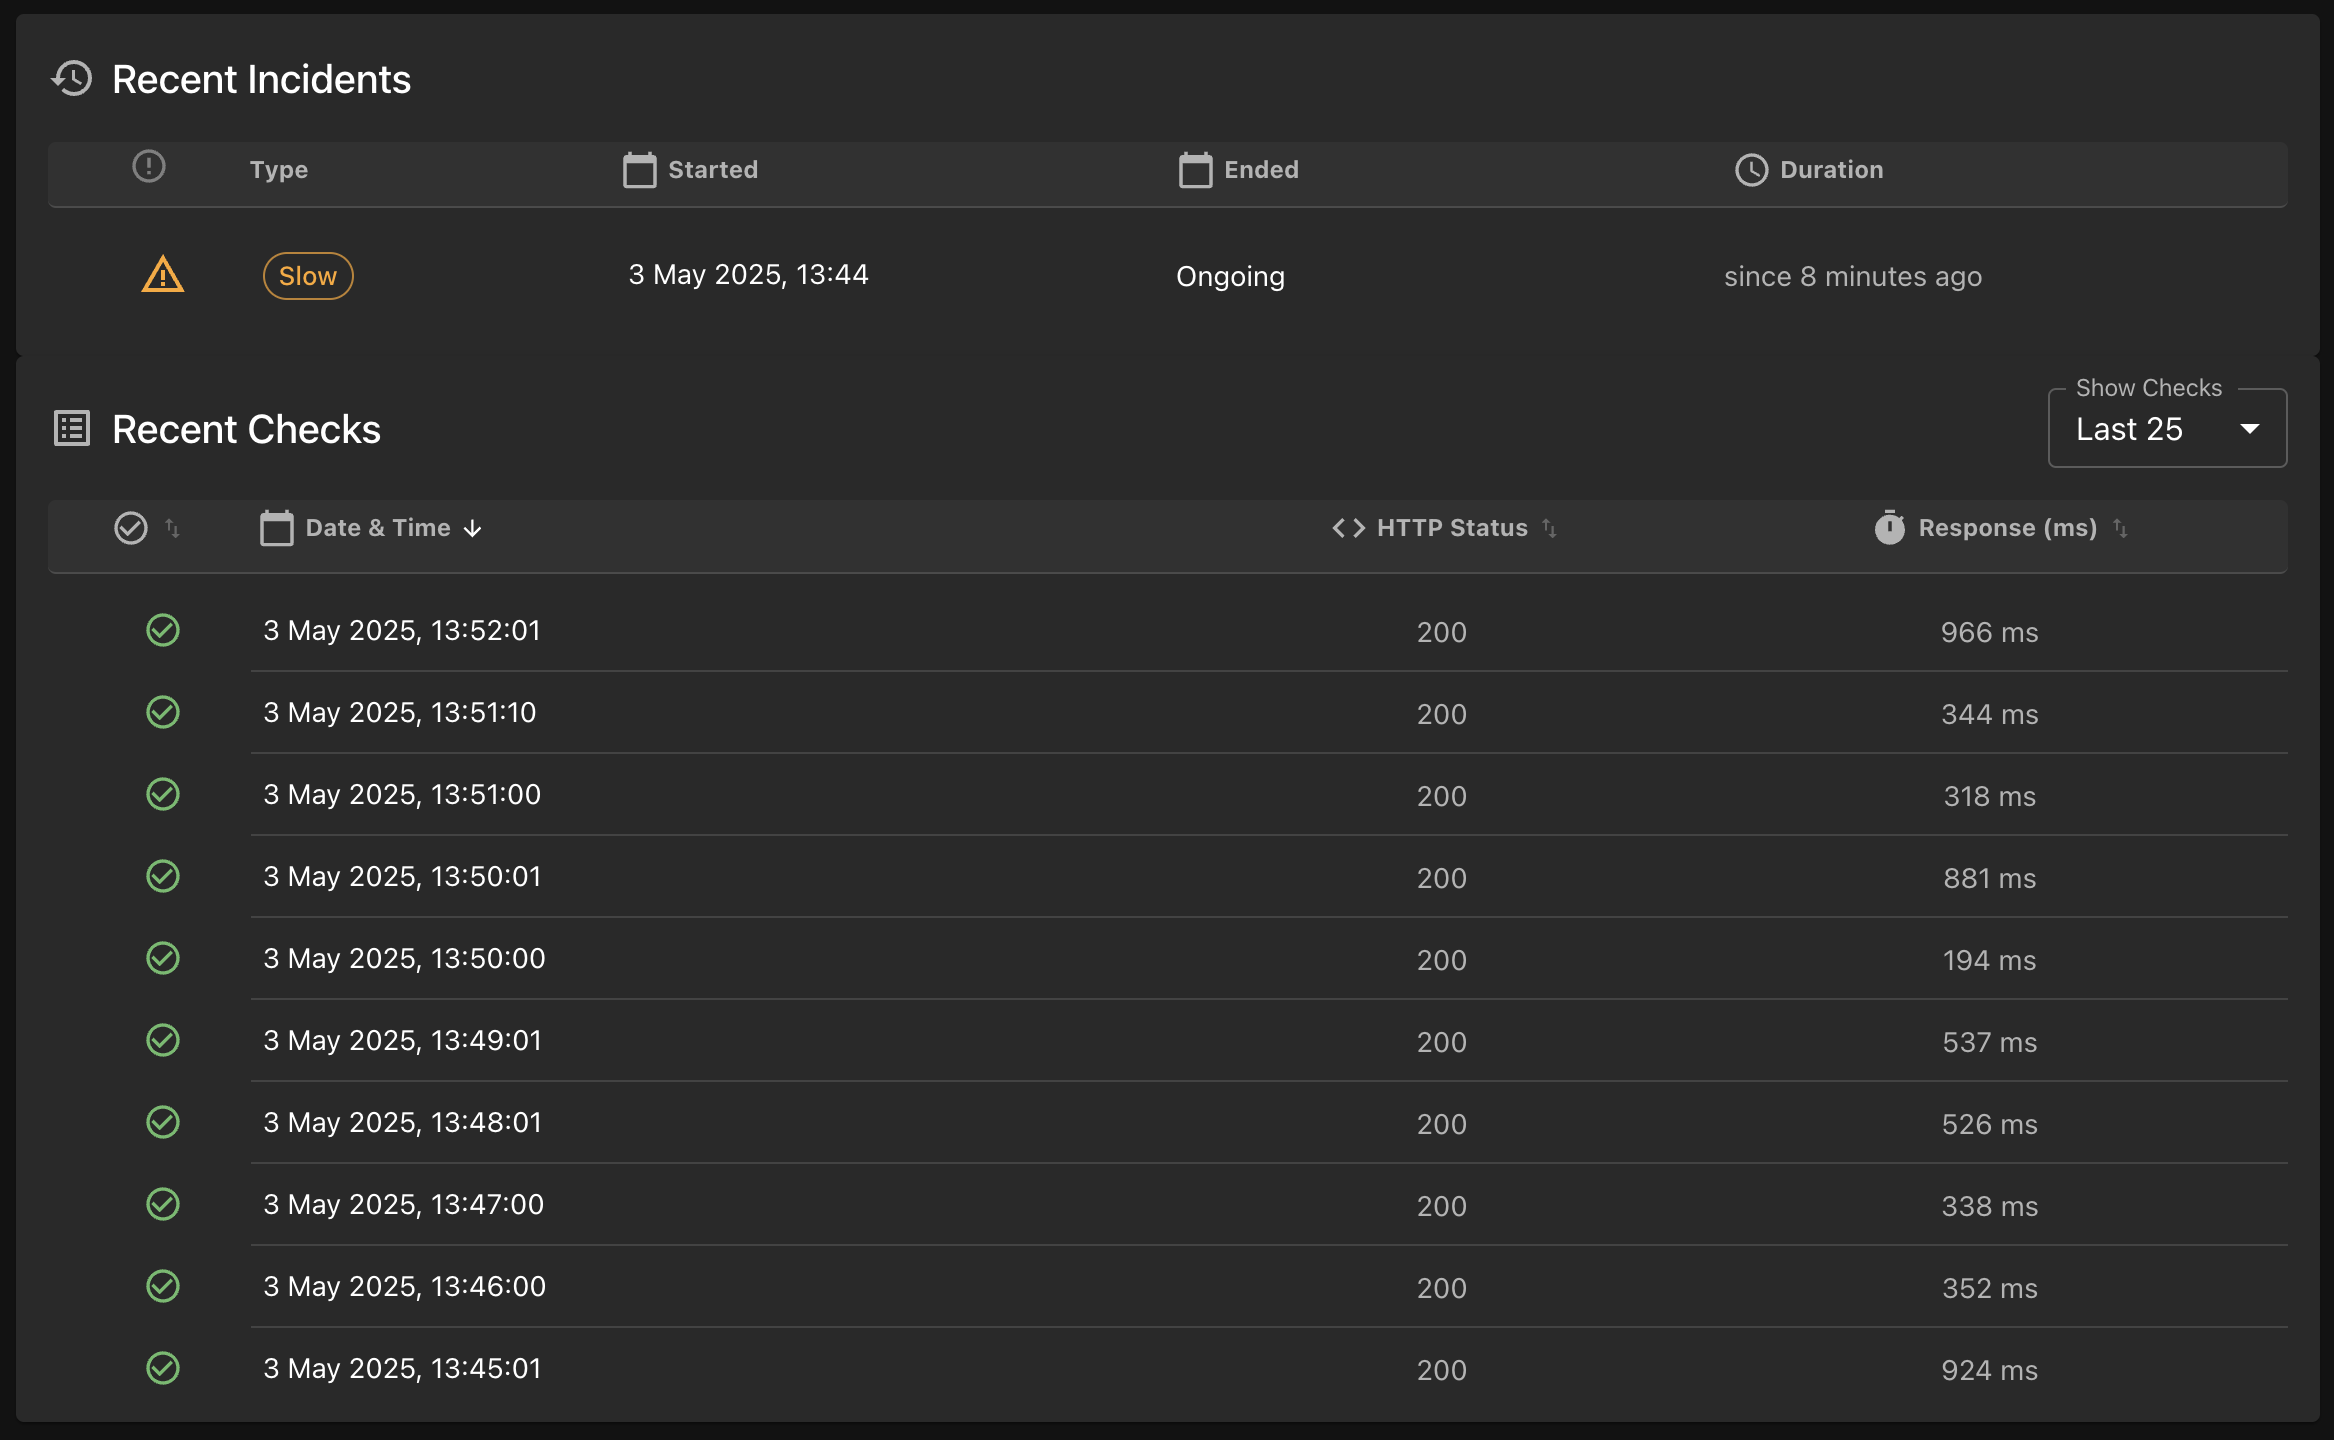
\includegraphics[width=1\linewidth]{figures/websiteDetails_bottom.png}
    \caption{Enter Caption}
    \label{fig:enter-label}
\end{figure}


%diskutere om disse her faktisk skal tas med I forhold til designvalg
\subsubsection{Incident list component}



\subsection{Requirement Fulfillment}

The application fulfilled nearly all high-priority functional and non-functional requirements from Tables~\ref{tab:functional_reqs_refined} and~\ref{tab:nonfunctional_reqs_refined}:

\begin{itemize}
    \item \textbf{Fully fulfilled:} F.1–F.4, F.6–F.8, NF.1–NF.3.
    \item \textbf{Partially fulfilled:} 
        \begin{itemize}
            \item F.5 – User authentication was implemented, but support for multi-role access (e.g., admin vs. viewer) was not.
            \item F.9 – Users can adjust check intervals, but the server does not enforce hard limits.
            \item NF.4 – The codebase is documented, but not extensively.
        \end{itemize}
    \item \textbf{Not implemented:} NF.5 – The system layout is responsive, but mobile-specific testing and optimizations were limited.
\end{itemize}

An additional requirement, F.11, was introduced during testing to track website incidents. This feature was implemented successfully and provided additional clarity for users.




\section{Summary of Development Process} 
This chapter described how user and stakeholder needs were translated into a working monitoring system through iterative development, prototyping, testing, and refinement. The technology stack, implementation strategies, and evaluation results collectively demonstrate a system that meets most core requirements and reflects key principles of usability, maintainability, and responsiveness.